\documentclass[12pt,a4paper,twoside]{article}

% Packages
\usepackage[margin=1in]{geometry}
\usepackage{cite}
\usepackage{amsmath,amssymb,amsfonts}
\usepackage{graphicx}
\usepackage{textcomp}
\usepackage{xcolor}
\usepackage[hidelinks]{hyperref}
\usepackage{listings}
\usepackage{titlesec}
\usepackage{tikz}
\usepackage{booktabs}
\usepackage{float}
\usepackage{fancyhdr}
\usepackage[font=small,labelfont=bf]{caption}
\usepackage{subcaption}
\usepackage{algorithm}
\usepackage{algpseudocode}
\usetikzlibrary{shapes.geometric, arrows.meta, positioning, calc, fit}

% Graphics path - figures are stored in results/figures
\graphicspath{{../results/figures/}}

% Header/footer setup
\pagestyle{fancy}
\fancyhf{}
\fancyhead[LE]{Reinforcement Learning Applied to the Snake Game}
\fancyhead[RO]{Al-Amri, Al-Ubejdij, Al-Moslemani, Humaid, Aldous, Gavankar}
\fancyfoot[C]{\thepage}
\renewcommand{\headrulewidth}{0.4pt}

% No paragraph indentation
\setlength{\parindent}{0pt}
\setlength{\parskip}{6pt}

% Prevent LaTeX from stretching vertical space to fill pages
\raggedbottom

% Document metadata
\def\BibTeX{{\rm B\kern-.05em{\sc i\kern-.025em b}\kern-.08em
    T\kern-.1667em\lower.7ex\hbox{E}\kern-.125emX}}

\begin{document}

\title{Reinforcement Learning Applied to the Snake Game\\
\large ECEN 446 Course Project\\[1em]
\normalsize Instructor: Dr. Joseph Boutros}

\author{
Elyas Al-Amri \and
Ejmen Al-Ubejdij \and
Ahmad Al-Moslemani \and
Marwan Humaid \and
Hamad Aldous \and
Umair Gavankar
}

\date{\today}

\maketitle

% Table of contents on separate page
\newpage
\setcounter{tocdepth}{2}
\tableofcontents
\newpage

%==============================================================================
% ABSTRACT
%==============================================================================
\begin{abstract}
We investigate reinforcement learning techniques for the classic Snake game, implementing Deep Q-Networks (DQN) with enhancements (Double, Dueling, PER, Noisy, Rainbow) and policy gradient methods (PPO). Our key finding is that state representation matters more than algorithm choice: flood-fill features that measure reachable free space double average scores compared to basic features (35.51 vs 17.54 for PPO), reducing entrapment deaths from 80\% to 42\%. PPO consistently outperforms DQN variants in both sample efficiency and final performance. For competitive two-snake training, direct co-evolution fails due to exploration collapse, but curriculum learning with progressively harder opponents produces capable agents. In head-to-head competition after 10M training steps, curriculum-trained agents show Big network dominance (47\% vs 32\% win rate), while direct PPO co-evolution surprisingly favors smaller networks (55\% vs 19\%). Models trained on 10x10 grids generalize to other sizes without retraining. GPU-accelerated vectorized environments enable parallel training across 256 simultaneous instances.
\end{abstract}

%==============================================================================
% SECTION 1: INTRODUCTION
%==============================================================================
\section{Introduction}

The Snake game presents an appealing testbed for reinforcement learning research. Despite simple rules (navigate a grid, eat food, avoid collisions), the game poses genuine challenges: sparse rewards, a growing body that constrains movement, and the risk of self-entrapment. These characteristics make Snake useful for studying state representation design, algorithm selection, and training stability without the complexity of continuous control or high-dimensional observation spaces.

\subsection{Problem Statement and Motivation}

This project develops RL agents for both single-snake and competitive two-snake environments. The single-snake setting allows systematic comparison of algorithms and state representations. The two-snake variant introduces multi-agent challenges: non-stationarity as opponent policies evolve, credit assignment when outcomes depend on both agents, and the risk of exploration collapse where agents learn to avoid each other rather than compete \cite{lowe2017multi}.

A key design goal is grid-size independence. Rather than learning from raw pixels (which ties the agent to a specific grid size), we use feature-based representations encoding relative spatial information. This allows agents trained on a $10 \times 10$ grid to generalize to other sizes without retraining.

\subsection{Contributions}

This work provides a systematic comparison of value-based and policy gradient methods on a controlled testbed, investigates state representation design through flood-fill spatial features, and develops curriculum learning strategies for competitive multi-agent training. All code, trained models, and experiments are available at \url{https://github.com/ElyasAmri/Snake-RL}.

%==============================================================================
% SECTION 2: BACKGROUND AND THEORY
%==============================================================================
\section{Background and Theory}

Reinforcement learning provides a mathematical framework for learning optimal behavior through trial and error. Unlike supervised learning, where correct actions are explicitly provided, RL agents must discover which actions yield the most reward by interacting with their environment. This section presents the theoretical foundations underlying modern RL algorithms, beginning with the formal framework of Markov Decision Processes and progressing through value-based and policy-based learning methods.

\subsection{Markov Decision Processes}

A Markov Decision Process (MDP) provides the mathematical foundation for formulating reinforcement learning problems \cite{sutton2018reinforcement}. An MDP is defined by a tuple $(\mathcal{S}, \mathcal{A}, P, R, \gamma)$ where $\mathcal{S}$ is the state space representing all possible states the environment can be in, $\mathcal{A}$ is the action space representing all possible actions the agent can take, $P: \mathcal{S} \times \mathcal{A} \times \mathcal{S} \rightarrow [0,1]$ is the state transition probability function where $P(s'|s,a)$ denotes the probability of transitioning to state $s'$ when taking action $a$ in state $s$, $R: \mathcal{S} \times \mathcal{A} \rightarrow \mathbb{R}$ is the reward function where $R(s,a)$ gives the immediate reward for taking action $a$ in state $s$, and $\gamma \in [0,1]$ is the discount factor determining the present value of future rewards.

The fundamental assumption of an MDP is the Markov property: the future state depends only on the current state and action, not on the history of past states and actions. Formally:
\begin{equation}
P(s_{t+1}|s_t, a_t, s_{t-1}, a_{t-1}, \ldots, s_0, a_0) = P(s_{t+1}|s_t, a_t)
\end{equation}

This memoryless property significantly simplifies the decision-making process, as the agent only needs to consider the current state rather than maintaining the complete history.

The goal of reinforcement learning is to find an optimal policy $\pi^*$ that maximizes the expected cumulative discounted reward, also called the \textbf{return}:
\begin{equation}
G_t = \sum_{k=0}^{\infty} \gamma^k R_{t+k+1}
\end{equation}
where $R_{t+k+1}$ is the reward received at time step $t+k+1$. The discount factor $\gamma$ serves two purposes: it ensures that the infinite sum converges (when $\gamma < 1$), and it expresses the preference for immediate rewards over delayed rewards.

\begin{figure}[H]
\centering
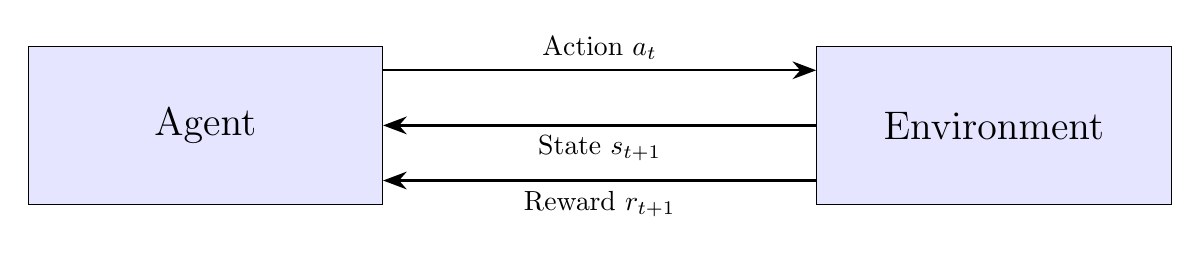
\begin{tikzpicture}[
    node distance=2.5cm,
    block/.style={rectangle, draw, minimum width=4.5cm, minimum height=2cm, align=center, fill=blue!10, font=\Large},
    arrow/.style={-{Stealth[length=3mm]}, thick}
]
    % Agent
    \node[block] (agent) {Agent};

    % Environment
    \node[block, right=5.5cm of agent] (env) {Environment};

    % Arrows - well spaced
    \draw[arrow] ([yshift=0.7cm]agent.east) -- node[above] {Action $a_t$} ([yshift=0.7cm]env.west);
    \draw[arrow] ([yshift=0cm]env.west) -- node[below] {State $s_{t+1}$} ([yshift=0cm]agent.east);
    \draw[arrow] ([yshift=-0.7cm]env.west) -- node[below] {Reward $r_{t+1}$} ([yshift=-0.7cm]agent.east);

\end{tikzpicture}
\caption{Agent-environment interaction in a Markov Decision Process.}
\label{fig:mdp}
\end{figure}

\subsection{Policy Function}

A \textbf{policy} $\pi$ defines the agent's behavior by specifying which action to take in each state. Policies can be deterministic or stochastic:

\textbf{Deterministic policy:} $\pi: \mathcal{S} \rightarrow \mathcal{A}$ maps states directly to actions. Given state $s$, the agent always takes action $a = \pi(s)$.

\textbf{Stochastic policy:} $\pi(a|s)$ represents the probability of selecting action $a$ when in state $s$. The agent samples actions according to this distribution, enabling exploration of different behaviors.

The choice between deterministic and stochastic policies has important implications. Stochastic policies are essential during learning to ensure exploration of the action space. They also arise naturally in multi-agent settings where predictable behavior can be exploited by opponents. However, for many single-agent tasks, the optimal policy is deterministic.

\subsection{Value Function (State-Value)}

The \textbf{state-value function} $V^\pi(s)$ estimates how good it is for an agent to be in a given state. It gives the expected return when starting in state $s$ and following policy $\pi$ thereafter:
\begin{equation}
V^\pi(s) = \mathbb{E}_\pi[G_t | s_t = s] = \mathbb{E}_\pi\left[\sum_{k=0}^{\infty} \gamma^k R_{t+k+1} \middle| s_t = s\right]
\end{equation}

The state-value function satisfies the \textbf{Bellman equation}:
\begin{equation}
V^\pi(s) = \sum_{a \in \mathcal{A}} \pi(a|s) \sum_{s' \in \mathcal{S}} P(s'|s,a)[R(s,a) + \gamma V^\pi(s')]
\end{equation}

The optimal state-value function is defined as the maximum value achievable over all policies:
\begin{equation}
V^*(s) = \max_\pi V^\pi(s)
\end{equation}

\subsection{Action-Value Function (Q-Function)}

The \textbf{action-value function} (or Q-function) $Q^\pi(s,a)$ estimates how good it is to take a particular action in a given state. It gives the expected return when starting in state $s$, taking action $a$, and following policy $\pi$ thereafter:
\begin{equation}
Q^\pi(s,a) = \mathbb{E}_\pi[G_t | s_t = s, a_t = a]
\end{equation}

The Q-function is particularly useful because it allows action selection without knowing the environment dynamics. Once we have the optimal Q-function $Q^*$, we can extract the optimal policy through:
\begin{equation}
\pi^*(s) = \arg\max_{a \in \mathcal{A}} Q^*(s,a)
\end{equation}

The optimal Q-function satisfies the \textbf{Bellman optimality equation}:
\begin{equation}
Q^*(s,a) = \sum_{s' \in \mathcal{S}} P(s'|s,a)\left[R(s,a) + \gamma \max_{a' \in \mathcal{A}} Q^*(s',a')\right]
\end{equation}

This greedy policy with respect to $Q^*$ is guaranteed to be optimal.

\subsection{On-Policy vs Off-Policy Learning}

A fundamental distinction in reinforcement learning is between on-policy and off-policy methods:

\textbf{On-policy methods} learn the value of the policy being used to make decisions. The agent collects experience using its current policy and updates that same policy based on those experiences. Examples include SARSA, A2C, and PPO. On-policy methods are generally more stable but less sample-efficient, as each experience can only be used once before the policy changes.

\textbf{Off-policy methods} learn the value of a different policy than the one being used to collect data. The agent follows a behavior policy (often exploratory) while learning about a target policy (often greedy). Examples include Q-learning and DQN. Off-policy methods can reuse past experiences through replay buffers, improving sample efficiency, but they can be less stable due to the distribution mismatch between behavior and target policies.

For our Snake game experiments, we employ both paradigms: DQN (off-policy) uses experience replay to learn from stored transitions, while PPO (on-policy) learns directly from freshly collected rollouts.

\subsection{Experience Replay}

Experience replay is a critical technique that enables stable training in deep reinforcement learning. The key insight is that training a neural network on consecutive samples from an agent's trajectory creates two problems: (1) consecutive samples are highly correlated, violating the i.i.d. assumption of stochastic gradient descent, and (2) the data distribution shifts as the policy improves, causing catastrophic forgetting of previously learned behaviors.

When training directly on sequential experiences, the network sees a stream of highly correlated transitions. For example, in Snake, consecutive states differ only slightly as the snake moves one cell. This correlation causes the gradient updates to be biased toward recent experiences, leading to oscillating or diverging Q-values. The network effectively ``forgets'' how to handle states it encountered earlier in training.

\begin{figure}[H]
\centering
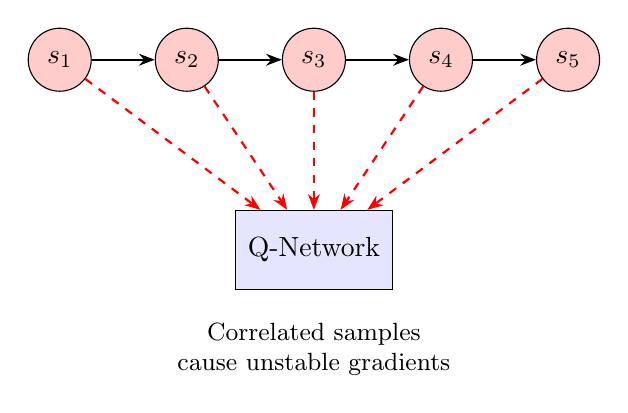
\begin{tikzpicture}[
    node distance=0.8cm,
    state/.style={circle, draw, minimum size=0.8cm, fill=red!20},
    arrow/.style={-{Stealth[length=2mm]}, thick},
    dashedarrow/.style={-{Stealth[length=2mm]}, thick, dashed}
]
    % Sequential states
    \node[state] (s1) {$s_1$};
    \node[state, right=of s1] (s2) {$s_2$};
    \node[state, right=of s2] (s3) {$s_3$};
    \node[state, right=of s3] (s4) {$s_4$};
    \node[state, right=of s4] (s5) {$s_5$};

    \draw[arrow] (s1) -- (s2);
    \draw[arrow] (s2) -- (s3);
    \draw[arrow] (s3) -- (s4);
    \draw[arrow] (s4) -- (s5);

    % Neural network
    \node[rectangle, draw, fill=blue!10, minimum width=2cm, minimum height=1cm, below=1.5cm of s3] (nn) {Q-Network};

    % Correlation indicator
    \draw[dashedarrow, red] (s1) -- (nn);
    \draw[dashedarrow, red] (s2) -- (nn);
    \draw[dashedarrow, red] (s3) -- (nn);
    \draw[dashedarrow, red] (s4) -- (nn);
    \draw[dashedarrow, red] (s5) -- (nn);

    % Label
    \node[below=0.3cm of nn, text width=6cm, align=center, font=\small] {Correlated samples cause unstable gradients};
\end{tikzpicture}
\caption{Without replay: sequential samples are correlated, causing training instability.}
\label{fig:no_replay}
\end{figure}

Experience replay addresses these issues by storing transitions $(s_t, a_t, r_{t+1}, s_{t+1})$ in a buffer and sampling mini-batches uniformly at random for training. This breaks temporal correlations and provides a more stationary data distribution. The buffer acts as a memory that allows reusing past experiences multiple times, improving sample efficiency.

\begin{figure}[H]
\centering
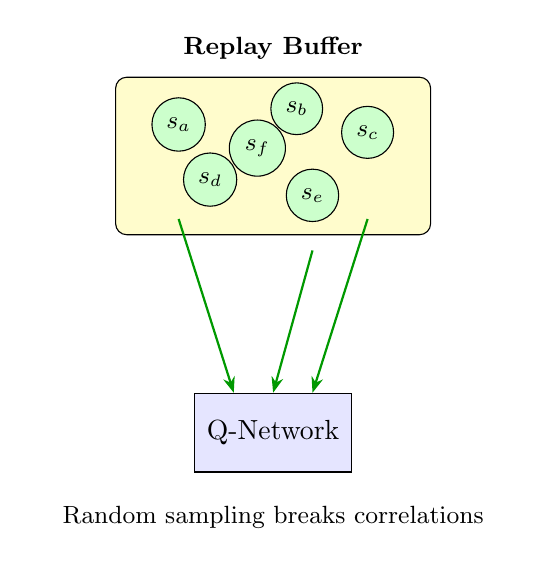
\begin{tikzpicture}[
    node distance=0.6cm,
    state/.style={circle, draw, minimum size=0.6cm, fill=green!20, font=\small},
    arrow/.style={-{Stealth[length=2mm]}, thick},
    dashedarrow/.style={-{Stealth[length=2mm]}, thick, dashed}
]
    % Replay buffer (cylinder-like)
    \node[rectangle, draw, fill=yellow!20, minimum width=4cm, minimum height=2cm, rounded corners] (buffer) {};
    \node[above=0.1cm of buffer.north, font=\small\bfseries] {Replay Buffer};

    % States inside buffer (scattered)
    \node[state] at (-1.2, 0.4) {$s_a$};
    \node[state] at (0.3, 0.6) {$s_b$};
    \node[state] at (1.2, 0.3) {$s_c$};
    \node[state] at (-0.8, -0.3) {$s_d$};
    \node[state] at (0.5, -0.5) {$s_e$};
    \node[state] at (-0.2, 0.1) {$s_f$};

    % Neural network
    \node[rectangle, draw, fill=blue!10, minimum width=2cm, minimum height=1cm, below=2cm of buffer] (nn) {Q-Network};

    % Random sampling arrows
    \draw[arrow, green!60!black] (-1.2, -0.8) -- ([xshift=-0.5cm]nn.north);
    \draw[arrow, green!60!black] (0.5, -1.2) -- (nn.north);
    \draw[arrow, green!60!black] (1.2, -0.8) -- ([xshift=0.5cm]nn.north);

    % Label
    \node[below=0.3cm of nn, text width=6cm, align=center, font=\small] {Random sampling breaks correlations};
\end{tikzpicture}
\caption{With replay: random sampling from buffer decorrelates training data.}
\label{fig:with_replay}
\end{figure}

The replay buffer typically stores the most recent $N$ transitions (e.g., $N = 100,000$), discarding older experiences as new ones arrive. This ensures the buffer contains a diverse set of experiences while remaining bounded in memory.

\subsection{Value-Based Methods}

Value-based methods learn the optimal value function and derive a policy from it. The foundational algorithm in this category is Q-learning \cite{watkins1992q}, which updates Q-values using:
\begin{equation}
Q(s_t, a_t) \leftarrow Q(s_t, a_t) + \alpha \left[R_{t+1} + \gamma \max_{a} Q(s_{t+1}, a) - Q(s_t, a_t)\right]
\end{equation}
where $\alpha$ is the learning rate. The term in brackets is the temporal difference (TD) error, measuring the discrepancy between the current estimate and the bootstrapped target.

For problems with large or continuous state spaces, tabular methods become infeasible. Deep Q-Networks (DQN) address this limitation by using deep neural networks as function approximators for the Q-function \cite{mnih2015human}. DQN introduces two critical innovations that stabilize training. \textbf{Experience replay} stores transitions $(s_t, a_t, r_{t+1}, s_{t+1})$ in a replay buffer and samples mini-batches uniformly for training, breaking temporal correlations and improving sample efficiency. The \textbf{target network} maintains a separate copy of the Q-network with parameters $\theta^-$ that are periodically synchronized with the main network, preventing the instability that arises from chasing a constantly moving target.

The DQN loss function is:
\begin{equation}
L(\theta) = \mathbb{E}_{(s,a,r,s') \sim \mathcal{D}}\left[\left(r + \gamma \max_{a'} Q(s',a';\theta^-) - Q(s,a;\theta)\right)^2\right]
\end{equation}

Several improvements to the basic DQN algorithm have been proposed. \textbf{Double DQN} \cite{van2016deep} addresses the overestimation bias by decoupling action selection from action evaluation, using the online network to select actions and the target network to evaluate them. \textbf{Dueling DQN} \cite{wang2016dueling} separates the Q-function into value and advantage streams: $Q(s,a) = V(s) + A(s,a) - \frac{1}{|\mathcal{A}|}\sum_{a'} A(s,a')$, enabling the network to learn state values independently of action advantages. \textbf{Prioritized Experience Replay} \cite{schaul2016prioritized} samples transitions based on their TD error magnitude, focusing learning on the most informative experiences. \textbf{Noisy Networks} \cite{fortunato2018noisy} replace deterministic layers with noisy ones, providing state-dependent exploration without requiring epsilon-greedy schedules.

\begin{figure}[H]
\centering
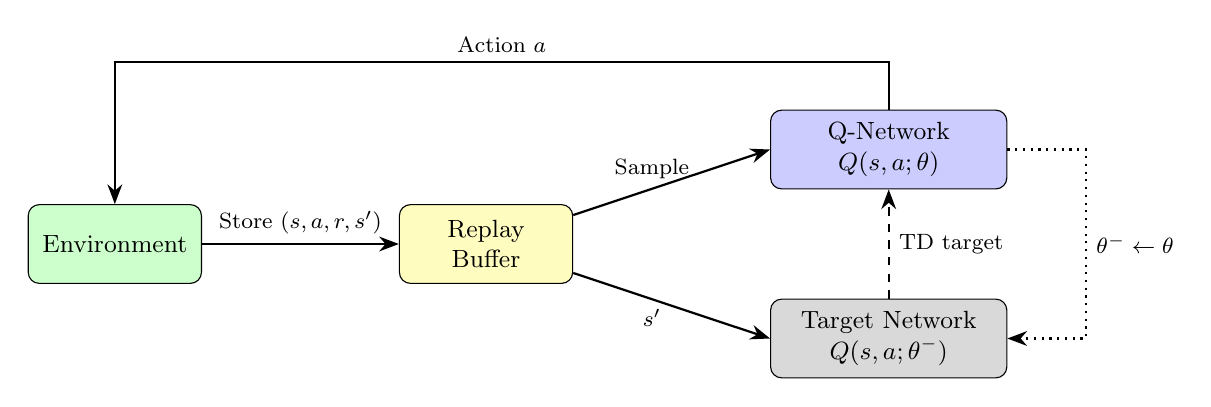
\begin{tikzpicture}[
    node distance=2cm,
    block/.style={rectangle, draw, rounded corners, minimum width=2.2cm, minimum height=1cm, align=center, font=\small},
    netblock/.style={rectangle, draw, rounded corners, minimum width=3cm, minimum height=1cm, align=center, font=\small},
    arrow/.style={-{Stealth[length=2.5mm]}, thick}
]
    % Horizontal layout: Environment -> Replay Buffer -> Networks
    \node[block, fill=green!20] (env) {Environment};
    \node[block, fill=yellow!25, right=2.5cm of env] (buffer) {Replay\\Buffer};

    % Networks stacked vertically on the right (increased spacing, same width)
    \node[netblock, fill=blue!20, right=2.5cm of buffer, yshift=1.2cm] (qnet) {Q-Network\\$Q(s,a;\theta)$};
    \node[netblock, fill=gray!30, right=2.5cm of buffer, yshift=-1.2cm] (target) {Target Network\\$Q(s,a;\theta^-)$};

    % === Main Data Flow ===

    % Environment stores transitions in buffer
    \draw[arrow] (env) -- node[above, font=\footnotesize] {Store $(s,a,r,s')$} (buffer);

    % Buffer feeds both networks
    \draw[arrow] (buffer) -- node[above, font=\footnotesize, pos=0.4] {Sample} (qnet.west);
    \draw[arrow] (buffer) -- node[below, font=\footnotesize, pos=0.4] {$s'$} (target.west);

    % Target provides TD target to Q-network
    \draw[arrow, dashed] (target.north) -- node[right, font=\footnotesize] {TD target} (qnet.south);

    % Q-network outputs action back to environment
    \draw[arrow] (qnet.north) -- ++(0, 0.6) -| node[above, font=\footnotesize, pos=0.25] {Action $a$} (env.north);

    % Periodic weight copy (loops around the right side, ending at target)
    \draw[arrow, dotted, thick] (qnet.east) -- ++(1.0, 0) |- node[right, font=\footnotesize, pos=0.25] {$\theta^- \leftarrow \theta$} (target.east);

\end{tikzpicture}
\caption{DQN training loop: experiences are stored in replay buffer, sampled for training, with target network providing stable Q-value targets.}
\label{fig:dqn}
\end{figure}

Table \ref{tab:dqn_variants} summarizes the DQN variants and their key improvements.

\begin{table}[H]
\centering
\caption{DQN Variants and Improvements}
\label{tab:dqn_variants}
\renewcommand{\arraystretch}{1.5}
\begin{tabular*}{\textwidth}{@{\extracolsep{\fill}}p{1.5cm}p{5cm}p{7cm}@{}}
\toprule
\textbf{Variant} & \textbf{Description} & \textbf{Key Equation} \\
\midrule
DQN & Base algorithm with experience replay and target network & $L(\theta) = \mathbb{E}[(r + \gamma \max_{a'} Q(s',a';\theta^-) - Q(s,a;\theta))^2]$ \\
Double & Decouples action selection from evaluation to reduce overestimation bias & $a^* = \arg\max_a Q(s',a;\theta)$, evaluate with $Q(s',a^*;\theta^-)$ \\
Dueling & Separates Q-function into value and advantage streams & $Q(s,a) = V(s) + A(s,a) - \frac{1}{|\mathcal{A}|}\sum_{a'} A(s,a')$ \\
PER & Samples transitions by TD error magnitude for focused learning & Priority $p_i = |\delta_i| + \epsilon$ \\
Noisy & Adds learnable noise to network weights for exploration & $y = (b + Wz)x$ where $z \sim \mathcal{N}(0,1)$ \\
Rainbow & Combines all improvements: Double, Dueling, PER, Noisy, N-step, Distributional & All of the above + distributional $Q(s,a) \sim \mathcal{Z}$ \\
\bottomrule
\end{tabular*}
\renewcommand{\arraystretch}{1.0}
\end{table}

\subsection{Policy Gradient Methods}

While value-based methods learn a value function and derive a policy from it, policy gradient methods directly parameterize and optimize the policy $\pi_\theta(a|s)$. The objective is to maximize the expected return:
\begin{equation}
J(\theta) = \mathbb{E}_{\tau \sim \pi_\theta}[G(\tau)]
\end{equation}

The policy gradient theorem \cite{williams1992simple} provides a way to compute gradients of this objective:
\begin{equation}
\nabla_\theta J(\theta) = \mathbb{E}_{\tau \sim \pi_\theta}\left[\sum_{t=0}^T \nabla_\theta \log \pi_\theta(a_t|s_t) G_t\right]
\end{equation}

The \textbf{REINFORCE} algorithm uses Monte Carlo estimation of this gradient, updating parameters after each complete episode. To reduce variance, a baseline $b(s_t)$ is subtracted from the return, with the state-value function $V(s_t)$ being a common choice. This leads to the advantage function $A(s,a) = Q(s,a) - V(s)$, which measures how much better an action is compared to the average.

Actor-Critic methods combine value-based and policy-based approaches. The actor (policy network) selects actions while the critic (value network) evaluates them, providing lower-variance gradient estimates. The Advantage Actor-Critic (A2C) algorithm \cite{mnih2016asynchronous} uses the TD error as an estimate of the advantage:
\begin{equation}
A(s_t, a_t) \approx r_{t+1} + \gamma V(s_{t+1}) - V(s_t)
\end{equation}

Proximal Policy Optimization (PPO) \cite{schulman2017proximal} has become one of the most popular RL algorithms due to its simplicity and effectiveness. Building on Trust Region Policy Optimization (TRPO) \cite{schulman2015trust}, PPO constrains policy updates to prevent large, destabilizing changes using a clipped surrogate objective:
\begin{equation}
L^{CLIP}(\theta) = \mathbb{E}_t\left[\min\left(r_t(\theta)A_t, \text{clip}(r_t(\theta), 1-\epsilon, 1+\epsilon)A_t\right)\right]
\end{equation}
where $r_t(\theta) = \frac{\pi_\theta(a_t|s_t)}{\pi_{\theta_{old}}(a_t|s_t)}$ is the probability ratio. The clipping prevents the policy from changing too drastically in a single update. PPO also uses Generalized Advantage Estimation (GAE) \cite{schulman2016high} to balance bias and variance in advantage estimates:
\begin{equation}
A_t^{GAE} = \sum_{l=0}^{\infty} (\gamma\lambda)^l \delta_{t+l}
\end{equation}
where $\delta_t = r_t + \gamma V(s_{t+1}) - V(s_t)$ is the TD error and $\lambda$ controls the trade-off.

\begin{figure}[H]
\centering
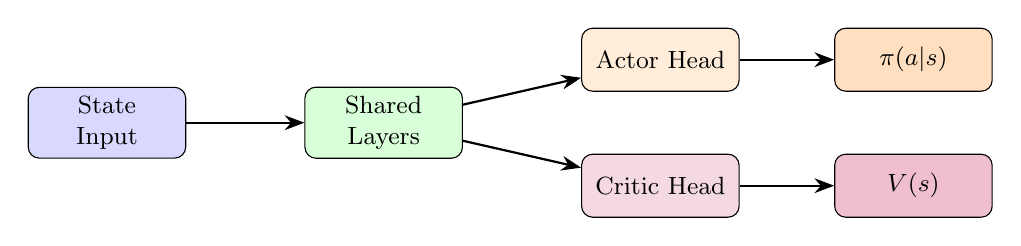
\begin{tikzpicture}[
    node distance=1.5cm,
    block/.style={rectangle, draw, rounded corners, minimum width=2cm, minimum height=0.8cm, align=center, font=\small},
    arrow/.style={-{Stealth[length=2.5mm]}, thick}
]
    % Horizontal layout: Input -> Shared -> Actor/Critic branches
    \node[block, fill=blue!15] (input) {State\\Input};
    \node[block, fill=green!15, right=1.5cm of input] (shared) {Shared\\Layers};

    % Actor branch (top)
    \node[block, fill=orange!15, right=1.5cm of shared, yshift=0.8cm] (actor) {Actor Head};
    \node[block, fill=orange!25, right=1.2cm of actor] (policy) {$\pi(a|s)$};

    % Critic branch (bottom)
    \node[block, fill=purple!15, right=1.5cm of shared, yshift=-0.8cm] (critic) {Critic Head};
    \node[block, fill=purple!25, right=1.2cm of critic] (value) {$V(s)$};

    % Arrows
    \draw[arrow] (input) -- (shared);
    \draw[arrow] (shared) -- (actor);
    \draw[arrow] (shared) -- (critic);
    \draw[arrow] (actor) -- (policy);
    \draw[arrow] (critic) -- (value);

\end{tikzpicture}
\caption{Actor-Critic architecture with shared layers, used in PPO and A2C.}
\label{fig:actor_critic}
\end{figure}

Table \ref{tab:policy_gradient_methods} summarizes the policy gradient methods we consider.

\begin{table}[H]
\centering
\caption{Policy Gradient Methods Comparison}
\label{tab:policy_gradient_methods}
\renewcommand{\arraystretch}{1.5}
\begin{tabular*}{\textwidth}{@{\extracolsep{\fill}}p{2cm}p{4.5cm}p{7cm}@{}}
\toprule
\textbf{Method} & \textbf{Description} & \textbf{Key Equation} \\
\midrule
REINFORCE & Monte Carlo policy gradient with episode returns & $\nabla J = \mathbb{E}[\sum_t \nabla \log \pi(a_t|s_t) G_t]$ \\
A2C & Advantage Actor-Critic with TD advantage estimation & $A(s_t,a_t) = r_{t+1} + \gamma V(s_{t+1}) - V(s_t)$ \\
PPO & Clipped surrogate objective for stable updates & $L = \min(r_t A_t, \text{clip}(r_t, 1\pm\epsilon) A_t)$ \\
TRPO & Trust region constraint on policy updates & $\max_\theta J(\theta)$ s.t. $D_{KL}(\pi_{\theta_{old}} || \pi_\theta) \leq \delta$ \\
\bottomrule
\end{tabular*}
\renewcommand{\arraystretch}{1.0}
\end{table}

%==============================================================================
% SECTION 3: IMPLEMENTATION
%==============================================================================
\section{Implementation}

This section describes our implementation of the Snake game environments and reinforcement learning infrastructure. We detail the code structure, GPU vectorization for efficient training, state representations, and action space design.

\subsection{Code Structure}

Our implementation follows a modular architecture organized into several components. The \texttt{core/} directory contains core modules including environments, neural networks, state representations, and utilities. Training scripts for each algorithm (DQN, PPO, A2C) reside in \texttt{scripts/training/}, while \texttt{scripts/visualizer/} provides visualization and recording tools. The \texttt{results/} directory stores trained weights, training data, and generated figures.

All environments follow the Gymnasium (OpenAI Gym) API standard, ensuring compatibility with standard RL libraries. The single-snake environment features a configurable grid (default $10 \times 10$) where the snake starts with length 3 at the center. Food appears randomly on empty cells, and episodes terminate upon collision with walls or the snake's body, or after a timeout of $2 \times \text{grid\_area}$ steps without collecting food.

For competitive scenarios, we implemented a two-snake environment where both snakes share the grid and compete for food. A round ends when one snake reaches a target food count or when a snake dies. The two-snake environment supports both classic (CPU-based) and vectorized (GPU-accelerated) implementations.

\subsection{GPU Vectorization}

A key contribution of our implementation is GPU-accelerated vectorized environments using PyTorch tensors. Instead of running a single game sequentially, we run 128-256 simultaneous games in parallel on the GPU. All game state (snake positions, food locations, directions) is stored as batched tensors, and game logic (collision detection, movement, reward computation) is implemented using vectorized tensor operations.

This vectorization enables significant throughput improvements by amortizing Python interpreter overhead across many parallel environments. With 256 simultaneous environments, we process approximately 10,000 episodes per minute on an RTX 4070, enabling extensive hyperparameter searches and longer training runs that would be time-prohibitive with sequential single-environment training. Training 2,000 PPO episodes with 256 parallel environments completes in approximately 3 minutes.

\subsection{State Representations}

State representation significantly impacts learning efficiency and final performance. We designed multiple representations with increasing sophistication, ranging from basic 11-dimensional feature vectors to comprehensive 24-dimensional representations.

The simplest representation uses 11 dimensions capturing immediate spatial awareness. This includes three binary danger indicators for collision risk in relative directions (straight, right, left), four binary food direction indicators showing whether food lies up, right, down, or left relative to the head, and four one-hot encoded features representing the snake's current absolute direction. This basic representation provides sufficient information for learning fundamental navigation skills.

Building on this foundation, we developed a 14-dimensional representation that adds flood-fill features. These three additional features measure the ratio of reachable cells in each relative direction using a breadth-first traversal similar to BFS. By computing how much free space is accessible from potential next positions, the agent can avoid moves leading to dead-ends or self-trapping situations. The flood-fill computation normalizes values by the maximum possible free cells, producing features in the range [0, 1].

Further extensions include a 19-dimensional selective representation that adds tail-related features (direction to tail and normalized distance), helping the snake follow its tail for safety in dense configurations. The most comprehensive 24-dimensional enhanced representation adds escape route counts, tail reachability via flood-fill, and snake length ratio. While providing rich information, this representation incurs higher computational cost that may not justify the marginal performance improvement.

For CNN-based approaches, we use a grid representation with 3 channels encoding head position, body position, and food position respectively. This raw grid input requires convolutional layers to extract spatial features but provides complete spatial information without hand-crafted feature engineering.

For competitive two-snake scenarios, we designed a 35-dimensional competitive representation. This combines self-awareness features (danger, food direction, current direction, flood-fill), opponent-awareness features (opponent body danger, head position relative to self, opponent direction, opponent length, distance to opponent, threat level), and competitive metrics (length difference, food count difference, food proximity advantage, space control ratio).

\begin{figure}[H]
\centering
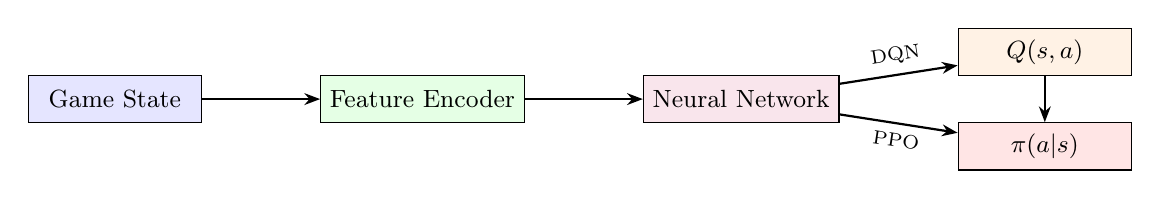
\begin{tikzpicture}[
    node distance=1cm,
    box/.style={rectangle, draw, minimum width=2.2cm, minimum height=0.6cm, align=center, font=\small},
    arrow/.style={-{Stealth[length=2mm]}, thick}
]
    % Horizontal flow: Game State -> Feature Encoder -> Neural Network -> Output
    \node[box, fill=blue!10] (state) {Game State};
    \node[box, fill=green!10, right=1.5cm of state] (encoder) {Feature Encoder};
    \node[box, fill=purple!10, right=1.5cm of encoder] (network) {Neural Network};

    % Q-value box (for DQN path)
    \node[box, fill=orange!10, right=1.5cm of network, yshift=0.6cm] (qvalue) {$Q(s,a)$};

    % Policy box (final output for both)
    \node[box, fill=red!10, right=1.5cm of network, yshift=-0.6cm] (policy) {$\pi(a|s)$};

    % Common path
    \draw[arrow] (state) -- (encoder);
    \draw[arrow] (encoder) -- (network);

    % DQN path: NN -> Q -> pi (labeled)
    \draw[arrow] (network) -- node[above, font=\scriptsize, sloped] {DQN} (qvalue);
    \draw[arrow] (qvalue) -- (policy);

    % PPO path: NN -> pi directly (labeled)
    \draw[arrow] (network) -- node[below, font=\scriptsize, sloped] {PPO} (policy);

\end{tikzpicture}
\caption{State representation pipeline: PPO outputs policy $\pi(a|s)$ directly, while DQN outputs Q-values $Q(s,a)$ which derive the policy.}
\label{fig:state_rep}
\end{figure}

\subsection{Environment Design}

The action space uses relative directions rather than absolute directions. STRAIGHT (0) continues in the current direction, RIGHT\_TURN (1) turns 90 degrees clockwise, and LEFT\_TURN (2) turns 90 degrees counter-clockwise. This relative action space offers several advantages over absolute directions (UP, DOWN, LEFT, RIGHT): the action space is reduced from 4 to 3 actions simplifying the learning problem, 180-degree turns (instant death) are impossible by construction, and the agent learns behaviors that generalize across all orientations. The relative encoding means the agent's decision depends only on what lies ahead, to the right, and to the left, not on absolute compass directions. This invariance reduces the effective state space the agent must learn.

The reward function guides learning behavior. For single-snake, we use food consumption (+10), collision/death (-10), and time penalty (-0.01 per step). The time penalty provides dense feedback encouraging efficient food collection rather than aimless wandering. Some experiments include distance-based shaping ($\pm 1$ for moving toward/away from food) to accelerate early learning. For competitive two-snake, rewards are more complex: food consumption gives +10, death results in -50 to -100 depending on configuration, winning the round yields +100, and the opponent dying while the agent survives provides +50. The step penalty is reduced or removed to focus on strategic play rather than speed.

\subsection{Network Architectures}

We implement two network architectures: MLP for feature-based inputs and CNN for grid-based inputs.

For MLP-based agents with feature input, we use two hidden layers with 128 neurons each and ReLU activations. Larger networks (256x256) are used for competitive scenarios requiring more capacity. The output layer produces Q-values (for DQN) or action logits (for policy gradient methods). For CNN-based agents with grid input, we use three convolutional layers (32, 64, 64 filters with 3x3 kernels), followed by a fully connected layer (256 neurons) and the output layer. Padding preserves spatial dimensions through the convolutional layers.

\begin{figure}[H]
\centering
\begin{subfigure}[c]{0.45\textwidth}
\centering
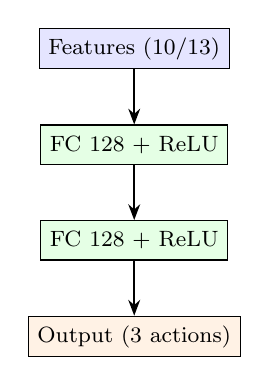
\begin{tikzpicture}[
    node distance=0.7cm,
    layer/.style={rectangle, draw, minimum width=2.2cm, minimum height=0.5cm, align=center, font=\footnotesize},
    arrow/.style={-{Stealth[length=2mm]}, thick}
]
    \node[layer, fill=blue!10] (input) {Features (10/13)};
    \node[layer, fill=green!10, below=of input] (fc1) {FC 128 + ReLU};
    \node[layer, fill=green!10, below=of fc1] (fc2) {FC 128 + ReLU};
    \node[layer, fill=orange!10, below=of fc2] (output) {Output (3 actions)};

    \draw[arrow] (input) -- (fc1);
    \draw[arrow] (fc1) -- (fc2);
    \draw[arrow] (fc2) -- (output);
\end{tikzpicture}
\caption{MLP for feature-based input.}
\label{fig:mlp_arch}
\end{subfigure}
\hfill
\begin{subfigure}[c]{0.45\textwidth}
\centering
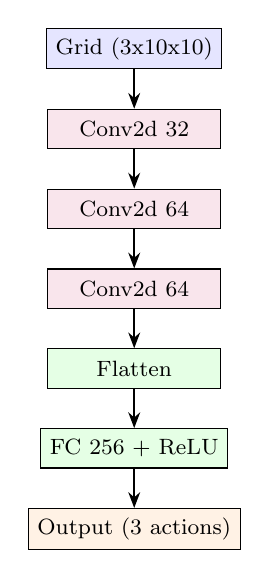
\begin{tikzpicture}[
    node distance=0.5cm,
    layer/.style={rectangle, draw, minimum width=2.2cm, minimum height=0.5cm, align=center, font=\footnotesize},
    arrow/.style={-{Stealth[length=2mm]}, thick}
]
    \node[layer, fill=blue!10] (input) {Grid (3x10x10)};
    \node[layer, fill=purple!10, below=of input] (conv1) {Conv2d 32};
    \node[layer, fill=purple!10, below=of conv1] (conv2) {Conv2d 64};
    \node[layer, fill=purple!10, below=of conv2] (conv3) {Conv2d 64};
    \node[layer, fill=green!10, below=of conv3] (flatten) {Flatten};
    \node[layer, fill=green!10, below=of flatten] (fc) {FC 256 + ReLU};
    \node[layer, fill=orange!10, below=of fc] (output) {Output (3 actions)};

    \draw[arrow] (input) -- (conv1);
    \draw[arrow] (conv1) -- (conv2);
    \draw[arrow] (conv2) -- (conv3);
    \draw[arrow] (conv3) -- (flatten);
    \draw[arrow] (flatten) -- (fc);
    \draw[arrow] (fc) -- (output);
\end{tikzpicture}
\caption{CNN for grid-based input.}
\label{fig:cnn_arch}
\end{subfigure}
\caption{Network architectures: (a) MLP with two hidden layers for feature-based state representation, (b) CNN with three convolutional layers for grid-based state representation.}
\label{fig:network_archs}
\end{figure}

Although CNNs are well-suited for spatial feature detection and could theoretically scale better to larger grid sizes by leveraging GPU parallelism for convolution operations, in practice CNNs are slower to run than MLPs with hand-crafted features. The convolutional operations add computational overhead that outweighs their benefits for our relatively small $10 \times 10$ grid. For this problem size, the MLP with flood-fill features provides both better performance and faster inference.

PPO uses separate actor and critic networks, or a shared backbone with separate heads. The actor outputs action logits processed through softmax for action probabilities. The critic outputs a single scalar value estimate.

To contextualize RL agent performance, we implemented several deterministic baseline algorithms. The random baseline selects actions uniformly at random, providing a lower bound on expected performance. The greedy food baseline uses A* pathfinding to navigate toward the nearest food, representing a simple but effective heuristic. The shortest path baseline employs Dijkstra's algorithm considering both walls and the snake's body as obstacles, representing near-optimal navigation when sufficient free space exists. These baselines establish performance benchmarks against which learning algorithms can be compared.

\subsection{Training Procedures}

We implemented training scripts for all algorithms with consistent interfaces and configurable hyperparameters. Table \ref{tab:hyperparameters} summarizes key hyperparameters.

\begin{table}[H]
\centering
\caption{Training Hyperparameters}
\label{tab:hyperparameters}
\begin{tabular}{lcc}
\toprule
\textbf{Parameter} & \textbf{DQN} & \textbf{PPO} \\
\midrule
Learning rate & 0.001 & 0.0003 \\
Discount factor ($\gamma$) & 0.99 & 0.99 \\
Batch size & 64 & 64 \\
Buffer/Rollout size & 100,000 & 2,048 \\
Hidden layers & 128x128 & 128x128 \\
$\epsilon$ start/end & 1.0/0.01 & N/A \\
$\epsilon$ decay & 0.995 & N/A \\
Clip parameter & N/A & 0.2 \\
GAE $\lambda$ & N/A & 0.95 \\
Entropy coefficient & N/A & 0.01 \\
Target update freq & 1,000 steps & N/A \\
\bottomrule
\end{tabular}
\end{table}

For DQN variants, we train for 5,000-10,000 episodes with 256 parallel environments. Training uses Adam optimizer with gradient clipping (max norm 1.0). The replay buffer stores transitions and samples uniformly (or by priority for PER). The target network updates every 1,000 training steps.

For policy gradient methods, we collect rollouts of 2,048 steps across parallel environments, then perform multiple epochs (4-10) of mini-batch updates. PPO uses the clipped objective with value function and entropy bonuses. A2C uses simpler advantage estimation without clipping.

For two-snake curriculum training, we progress through five stages with increasing opponent difficulty. Each stage trains until a win rate threshold is achieved (70\% for static, 60\% for random, 55\% for greedy, 50\% for frozen) or a maximum step count is reached. The final co-evolution stage trains both agents simultaneously.

%==============================================================================
% SECTION 4: EXPERIMENTS
%==============================================================================
\section{Experiments}

This section presents our experimental results, organized to demonstrate the progression of our investigation. We begin with vanilla implementations of DQN and PPO, then explore DQN variants and advanced algorithms. We investigate death causes to understand failure modes, introduce flood-fill features as a solution, study reward system modifications, and demonstrate grid size generalization. Finally, we present results from the competitive two-snake environment.

\subsection{Vanilla DQN and PPO}

We first establish baseline performance with standard implementations of DQN and PPO using basic features (danger indicators, food direction, current direction). Both algorithms were trained with 256 parallel environments on a $10 \times 10$ grid. DQN was trained for 3,000 episodes, while PPO achieved comparable results in 2,000 episodes due to its superior sample efficiency.

\textbf{Figure \ref{fig:dqn_results}} shows DQN training progression with basic features, demonstrating the characteristic learning curve with initial exploration phase followed by exploitation. \textbf{Figure \ref{fig:ppo_results}} shows PPO training, which exhibits faster convergence and more stable learning dynamics.

\begin{figure}[H]
\centering
\begin{subfigure}[b]{0.48\textwidth}
\centering
\includegraphics[width=\textwidth]{dqn_basic_scores.png}
\caption{DQN: 16-17 avg, 43 max score.}
\label{fig:dqn_results}
\end{subfigure}
\hfill
\begin{subfigure}[b]{0.48\textwidth}
\centering
\includegraphics[width=\textwidth]{ppo_basic_scores.png}
\caption{PPO: 17-18 avg, 38 max score.}
\label{fig:ppo_results}
\end{subfigure}
\caption{Training with basic features: DQN (3000 episodes) vs PPO (2000 episodes).}
\label{fig:basic_training}
\end{figure}

PPO consistently outperforms DQN in sample efficiency, achieving comparable or better final scores in fewer episodes. This advantage stems from PPO's on-policy learning with entropy regularization, which maintains exploration throughout training, unlike DQN's decaying epsilon-greedy strategy.

\subsection{DQN Variants}

We evaluated several DQN improvements to understand their individual contributions. Double DQN reduces overestimation bias by decoupling action selection from evaluation. Dueling DQN separates value and advantage streams for better state evaluation. Prioritized Experience Replay (PER) focuses learning on high-error transitions. Noisy Networks replaces epsilon-greedy with learnable exploration.

In our experiments, Double DQN provided the most consistent improvement, reducing Q-value overestimation that can destabilize learning. Dueling DQN showed benefits in states where most actions have similar value. PER accelerated early learning but required careful tuning of priority parameters. Noisy networks eliminated the need for epsilon scheduling but required longer training to learn appropriate exploration levels.

Rainbow DQN \cite{hessel2018rainbow} combines multiple DQN improvements into a single agent: Double Q-learning for reduced overestimation, Dueling architecture for better value estimation, Prioritized Experience Replay for efficient sampling, Noisy networks for exploration, and Distributional RL for modeling return distributions. Our implementation uses 51 atoms with support range [-20, 500] to capture the full reward distribution. In our experiments with basic features, Rainbow DQN achieves an average score of 17.94 $\pm$ 6.59, comparable to other DQN variants. The combination of improvements provides stability but does not dramatically outperform simpler variants in our Snake environment, likely because the relatively simple state space does not fully leverage Rainbow's distributional modeling capabilities.

\subsection{Death Cause Analysis}

Understanding why agents die provides insight into failure modes. We categorize deaths into three types: wall collisions (hitting the grid boundary), self-collisions (hitting the snake's own body during normal movement), and entrapments (the snake boxes itself in with no valid escape moves).

\textbf{Figures \ref{fig:dqn_deaths}} and \textbf{\ref{fig:ppo_deaths}} show cumulative death causes over training episodes with basic features.

\begin{figure}[H]
\centering
\begin{subfigure}[b]{0.48\textwidth}
\centering
\includegraphics[width=\textwidth]{dqn_basic_deaths.png}
\caption{DQN: entrapment dominates (67\%).}
\label{fig:dqn_deaths}
\end{subfigure}
\hfill
\begin{subfigure}[b]{0.48\textwidth}
\centering
\includegraphics[width=\textwidth]{ppo_basic_deaths.png}
\caption{PPO: entrapment dominates (80\%).}
\label{fig:ppo_deaths}
\end{subfigure}
\caption{Cumulative death causes with basic features.}
\label{fig:basic_deaths}
\end{figure}

With basic features, entrapment is the dominant death cause at 67-80\% of deaths, indicating that agents without spatial awareness frequently maneuver into positions from which escape is impossible. Notably, PPO's wall and self-collision curves flatten toward the end of training, indicating the agent has essentially learned to avoid these immediate dangers completely, yet it still dies frequently from entrapment, which requires longer-term spatial planning. This motivates the flood-fill feature engineering described in the next section.

\subsection{Flood-Fill Feature Engineering}

The flood-fill feature gives the agent spatial awareness about reachable free space. For each potential next position, we compute the ratio of cells reachable via breadth-first flood-fill traversal (see Algorithm~\ref{alg:floodfill} in Appendix~\ref{app:floodfill}). The result is a value in [0, 1] representing the fraction of free space reachable from that direction. Low values indicate potential dead-ends; high values indicate open space.

\textbf{Figures \ref{fig:dqn_flood}} and \textbf{\ref{fig:ppo_flood}} demonstrate the dramatic improvement in training scores from flood-fill features compared to the basic feature results shown in \textbf{Figures \ref{fig:dqn_results}} and \textbf{\ref{fig:ppo_results}}.

\begin{figure}[H]
\centering
\begin{subfigure}[b]{0.48\textwidth}
\centering
\includegraphics[width=\textwidth]{dqn_flood-fill_scores.png}
\caption{DQN: 24-27 avg, 56 max score.}
\label{fig:dqn_flood}
\end{subfigure}
\hfill
\begin{subfigure}[b]{0.48\textwidth}
\centering
\includegraphics[width=\textwidth]{ppo_flood-fill_scores.png}
\caption{PPO (2K episodes): 35-37 avg, 58 max.}
\label{fig:ppo_flood}
\end{subfigure}
\caption{Training with flood-fill features: dramatic improvement over basic features.}
\label{fig:flood_training}
\end{figure}

Table \ref{tab:representation_comparison} compares performance with and without flood-fill features. The flood-fill representation improves average scores by 46\% for DQN and 102\% for PPO, representing the single most impactful improvement in our experiments.

\begin{table}[H]
\centering
\caption{Single-Snake Performance: Basic vs Flood-fill Features}
\label{tab:representation_comparison}
\begin{tabular}{llcccc}
\toprule
\textbf{Algorithm} & \textbf{Features} & \textbf{Avg Score} & \textbf{Std} & \textbf{Max} & \textbf{Entrap \%} \\
\midrule
DQN & Basic & 16.78 & 6.91 & 43 & 68\% \\
DQN & Flood-fill & 24.53 & 10.98 & 56 & 42\% \\
PPO & Basic & 17.54 & 5.80 & 38 & 84\% \\
PPO & Flood-fill & 35.51 & 6.65 & 58 & 37\% \\
\bottomrule
\end{tabular}
\end{table}

With flood-fill, entrapment drops from 67-80\% to 42-52\% of deaths, explaining the doubled scores. \textbf{Figures \ref{fig:dqn_flood_deaths}} and \textbf{\ref{fig:ppo_flood_deaths}} show this improvement.

\begin{figure}[H]
\centering
\begin{subfigure}[b]{0.48\textwidth}
\centering
\includegraphics[width=\textwidth]{dqn_flood-fill_deaths.png}
\caption{DQN: entrapment reduced to 42\%.}
\label{fig:dqn_flood_deaths}
\end{subfigure}
\hfill
\begin{subfigure}[b]{0.48\textwidth}
\centering
\includegraphics[width=\textwidth]{ppo_flood-fill_deaths.png}
\caption{PPO: entrapment reduced to 52\%.}
\label{fig:ppo_flood_deaths}
\end{subfigure}
\caption{Cumulative death causes with flood-fill features.}
\label{fig:flood_deaths}
\end{figure}

An unexpected observation from the flood-fill experiments is the reintroduction of wall and self-collision deaths. With basic features, entrapment dominated (67-84\% of deaths), but with flood-fill, wall and self-collisions become more prominent again. This suggests that while flood-fill successfully addresses spatial awareness for avoiding dead-ends, the agent may become overconfident in tight spaces or take riskier paths. This motivated our investigation into reward system modifications to further reduce these preventable deaths.

\subsection{Reward System Modification}

We investigated whether reward engineering could reduce deaths beyond what flood-fill achieves. Specifically, we studied the death penalty hyperparameter, testing values from -10 to -100. This parameter controls how strongly the agent is penalized for dying, potentially affecting the exploration-exploitation trade-off and learned risk tolerance.

Table \ref{tab:ppo_penalty} shows PPO results across death penalties for both feature sets. With basic features, the penalty has moderate impact, with all values producing similar average scores in the 18-20 range. With flood-fill features, scores are consistently higher, with the -100 penalty producing the best average score of 39.74.

\begin{table}[H]
\centering
\caption{PPO Death Penalty Study: Basic vs Flood-fill Features}
\label{tab:ppo_penalty}
\begin{tabular}{ccccc}
\toprule
 & \multicolumn{2}{c}{\textbf{Basic Features}} & \multicolumn{2}{c}{\textbf{Flood-fill Features}} \\
\cmidrule(lr){2-3} \cmidrule(lr){4-5}
\textbf{Death Penalty} & \textbf{Avg} & \textbf{Max} & \textbf{Avg} & \textbf{Max} \\
\midrule
-10 & 19.48 & \textbf{45} & 35.08 & 59 \\
-20 & 18.40 & \textbf{45} & 35.91 & 60 \\
-30 & 18.25 & 40 & 36.98 & \textbf{64} \\
-40 & 19.30 & 41 & 37.52 & 59 \\
-50 & 19.25 & 40 & 36.76 & 58 \\
-100 & \textbf{19.93} & 39 & \textbf{39.74} & 56 \\
\bottomrule
\end{tabular}
\end{table}

The death penalty has less impact than state representation. Across all tested values, the difference in average score is at most 4-5 points, while switching from basic to flood-fill features provides an 18-point improvement. This suggests that investing effort in state representation design yields greater returns than hyperparameter tuning.

\subsection{Grid Size Generalization}

A key advantage of our feature-based state representation is grid-size independence. Because the features encode relative spatial information (danger indicators, food direction, flood-fill ratios) rather than absolute positions, an agent trained on a $10 \times 10$ grid can generalize to larger or smaller grids without retraining.

To validate this, we trained a DQN agent with flood-fill features on a $10 \times 10$ grid for 5,000 episodes, then evaluated its performance on $8 \times 8$, $10 \times 10$, $15 \times 15$, and $20 \times 20$ grids without any additional training. Table \ref{tab:grid_generalization} summarizes the results.

\begin{table}[H]
\centering
\caption{Grid Size Generalization: Model Trained on 10x10, Evaluated on Multiple Sizes}
\label{tab:grid_generalization}
\begin{tabular}{lcccc}
\toprule
\textbf{Grid Size} & \textbf{Avg Score} & \textbf{Max Score} & \textbf{Theoretical Max} & \textbf{\% of Max} \\
\midrule
$8 \times 8$ & 25.1 & 39 & 61 & 41.2\% \\
$10 \times 10$ (trained) & 34.8 & 54 & 97 & 35.9\% \\
$15 \times 15$ & 57.1 & 72 & 222 & 25.7\% \\
$20 \times 20$ & 55.2 & 71 & 397 & 13.9\% \\
\bottomrule
\end{tabular}
\end{table}

The results demonstrate successful generalization across grid sizes. Absolute scores actually increase on larger grids because the snake has more room to maneuver before facing space constraints. The percentage of theoretical maximum decreases for larger grids, which is expected since filling a larger grid requires longer survival and more strategic planning.

\begin{figure}[H]
\centering
\includegraphics[width=0.95\textwidth]{grid_size_generalization.png}
\caption{Grid size generalization: model trained on 10x10 transfers to other sizes.}
\label{fig:grid_generalization}
\end{figure}

The feature encoder only requires normalizing flood-fill values by the new grid's maximum free cells. All other features (danger indicators, food direction, current direction) remain unchanged, enabling zero-shot transfer to unseen grid sizes.

\subsection{Two-Snake Competitive Environment}

Competitive training proved more challenging than single-snake scenarios, requiring curriculum learning for stable performance. In the two-snake environment, both agents share the grid and compete for food, introducing non-stationarity as each agent's policy evolves during training.

We investigate whether larger networks produce better competitive agents by training two agents with different network capacities: a Big network with 256x256 hidden layers (131,000+ parameters) and a Small network with 128x128 hidden layers (33,000+ parameters). The hypothesis is that competitive scenarios require more representational capacity to model opponent behavior, strategic planning, and multi-objective optimization (food collection vs. survival vs. blocking opponent).

Competitive multi-agent RL introduces several challenges absent in single-agent settings. Non-stationarity arises because the opponent's policy changes during training, violating the stationarity assumption of most RL algorithms. Credit assignment becomes difficult: when one snake dies, it is unclear whether this resulted from its own mistake or the opponent's skill. Reward design must balance food collection, survival, and competitive objectives. Finally, exploration collapse can occur when both agents converge to avoiding each other rather than competing.

Our initial approach was direct co-evolution: training both agents simultaneously from random initialization. This approach failed to produce capable agents. Both snakes learned to avoid the center of the grid and each other, resulting in passive play with neither agent collecting food efficiently.

The failure occurs because early in training, random policies cause frequent collisions. The agents learn that approaching the opponent is dangerous, but this learned avoidance prevents them from developing competitive food-collection strategies. \textbf{Figure \ref{fig:two_snake_training}} compares training curves across all three approaches.

\begin{figure}[H]
\centering
\begin{subfigure}[b]{0.48\textwidth}
\centering
\includegraphics[width=\textwidth]{two_snake_training_curves.png}
\caption{Training curves: direct co-evolution vs curriculum.}
\label{fig:two_snake_training}
\end{subfigure}
\hfill
\begin{subfigure}[b]{0.48\textwidth}
\centering
\includegraphics[width=\textwidth]{two_snake_curriculum_stages.png}
\caption{Curriculum progression through 5 stages.}
\label{fig:curriculum_stages}
\end{subfigure}
\caption{Two-snake competitive training comparison (10M steps).}
\label{fig:two_snake_combined}
\end{figure}

To address co-evolution failure, we employ a five-stage curriculum with progressively increasing opponent difficulty. Table \ref{tab:curriculum_stages} summarizes both the curriculum design and results. Each stage requires achieving both the minimum training steps and the win rate threshold before advancing. The greedy opponent using BFS pathfinding proved extremely challenging; our agent never exceeded 5\% win rate and was advanced via the max-steps safety limit. Despite this, the final co-evolution stage produced competitive performance with 74\% win rate.

\begin{table}[H]
\centering
\caption{Curriculum Learning: Design and Results (10M steps)}
\label{tab:curriculum_stages}
\begin{tabular}{clccccc}
\toprule
\textbf{Stage} & \textbf{Opponent} & \textbf{Min Steps} & \textbf{Threshold} & \textbf{Achieved} & \textbf{Avg Score} & \textbf{Notes} \\
\midrule
0 & Static & 1M & 70\% & 94\% & -- & Passed \\
1 & Random & 1M & 60\% & 95\% & -- & Passed \\
2 & Greedy & 2M & 5\% & 0\% & 0.1 vs 3.8 & Max-steps \\
3 & Frozen & 2M & 30\% & 30\% & 0.3 vs 3.0 & Passed \\
4 & Co-evolution & 3M & N/A & 74\% & 1.3 vs 0.2 & Passed \\
\bottomrule
\end{tabular}
\end{table}

After training, we evaluate each approach by running 100 head-to-head games between the Big (256x256) and Small (128x128) networks. Games are played on a 20x20 grid with target food count of 10. A game ends when one snake reaches the target, one snake dies (collision with wall, self, or opponent), or both snakes die simultaneously (draw). We compare three training approaches: DQN direct co-evolution, PPO direct co-evolution, and PPO with curriculum learning.

\begin{figure}[H]
\centering
\includegraphics[width=0.95\textwidth]{two_snake_final_competition.png}
\caption{Final competition: Big vs Small network across three training approaches.}
\label{fig:final_competition}
\end{figure}

Table \ref{tab:two_snake_competition} summarizes the final competition results. Training time and total steps vary significantly between approaches.

\begin{table}[H]
\centering
\caption{Two-Snake Competition Results: Direct Training vs Curriculum}
\label{tab:two_snake_competition}
\begin{tabular}{lccccc}
\toprule
\textbf{Method} & \textbf{Big Win} & \textbf{Small Win} & \textbf{Draw} & \textbf{Steps} & \textbf{Time} \\
\midrule
DQN Direct & 4\% & 3\% & 93\% & 10,000,000 & 23 min \\
PPO Direct & 19\% & 55\% & 26\% & 10,000,000 & 126 min \\
PPO Curriculum & 47\% & 32\% & 21\% & 9,267,200 & 130 min \\
\bottomrule
\end{tabular}
\end{table}

The results reveal surprising patterns in competitive training with extended training (10M steps). DQN co-evolution still fails with 93\% draws: agents learn passive avoidance rather than competitive food collection, even with 10x more training time.

Unexpectedly, PPO direct co-evolution favors the \textit{smaller} network: the Small (128x128) network wins 55\% of games versus only 19\% for the Big (256x256) network. This counterintuitive result suggests that larger networks may overfit or learn suboptimal strategies when both agents evolve simultaneously without curriculum guidance.

PPO Curriculum produces the expected outcome: the Big network wins 47\% versus Small's 32\%. While neither dominates completely, the curriculum approach successfully leverages the larger network's representational capacity, reversing the trend seen in direct co-evolution.

Key observations from competitive training include:

\begin{itemize}
\item DQN co-evolution fails regardless of training duration; 93\% draws indicate fundamental algorithm limitations
\item PPO direct co-evolution unexpectedly favors smaller networks (55\% vs 19\%), possibly due to overfitting in larger networks
\item Curriculum learning is essential for larger networks to leverage their capacity advantage (47\% vs 32\%)
\item Extended training (10M steps) reveals dynamics not visible in shorter runs
\end{itemize}

The curriculum approach is crucial for competitive scenarios: without it, larger networks may actually perform worse than smaller ones due to co-adaptation dynamics.

%==============================================================================
% SECTION 5: DISCUSSION
%==============================================================================
\section{Discussion}

This section synthesizes key insights from our experiments.

\subsection{Why State Representation Matters More Than Algorithms}

Our most striking finding is the dominance of state representation over algorithm choice. Switching from basic to flood-fill features provides an 18-point improvement, while the best algorithm (PPO) only outperforms the worst (standard DQN) by 4 points with identical features. Similarly, death penalty tuning yields at most 4-5 point variation. This hierarchy---representation > algorithm > hyperparameters---suggests that for spatial planning problems, engineering effort should prioritize state design.

The flood-fill feature succeeds because it directly encodes the information needed to solve the primary failure mode: entrapment. Basic features provide local obstacle detection but no global path information, leaving agents blind to dead-ends until trapped. Flood-fill transforms this into an observable quantity, enabling preemptive avoidance.

\subsection{The Entrapment Problem}

Death cause analysis reveals that 67-80\% of failures with basic features stem from self-entrapment---a strategic error, not a tactical one. The snake navigates correctly but plans poorly. Flood-fill reduces entrapment to 42-52\%, with wall and self-collision deaths increasing proportionally. This shift from strategic to tactical deaths indicates a qualitatively different learned policy: one that maintains escape routes rather than greedily pursuing food.

This insight has implications for reward design. Our death penalty study shows that penalizing deaths more heavily does not reduce entrapment---the agent cannot avoid what it cannot perceive. Differential penalties based on death type (higher for avoidable tactical errors, lower for strategic entrapment) could encourage agents to take calculated risks in confined spaces rather than accepting entrapment passively.

\subsection{Why Larger Networks Can Fail in Competition}

The counterintuitive result that smaller networks outperform larger ones in PPO direct co-evolution (55\% vs 19\%) challenges the assumption that more capacity is always beneficial. We hypothesize two mechanisms:

\textbf{Overfitting to opponent dynamics}: Larger networks may memorize opponent-specific patterns that become obsolete as the opponent's policy evolves, while smaller networks learn more generalizable strategies.

\textbf{Co-adaptation instability}: With more parameters, both networks can develop increasingly complex counter-strategies, leading to an arms race that destabilizes learning. Smaller networks may converge to simpler, more stable equilibria.

Curriculum learning breaks this dynamic by providing stable, non-adapting opponents during early training. The larger network's capacity becomes an advantage only after developing fundamental skills against fixed opponents.

\subsection{Lessons for Multi-Agent RL}

DQN's complete failure in competitive settings (93\% draws) versus PPO's partial success highlights a fundamental limitation of value-based methods in non-stationary environments. Q-learning assumes a stationary MDP, but competitive training violates this assumption as opponent policies change. PPO's on-policy updates may better handle this non-stationarity.

Credit assignment in competitive scenarios remains an open challenge. When one snake dies, attributing this to self-error versus opponent skill is inherently ambiguous. Curriculum learning partially addresses this by starting with deterministic opponents where credit assignment is unambiguous, gradually introducing complexity as the agent develops competence.

%==============================================================================
% SECTION 6: CONCLUSION
%==============================================================================
\section{Conclusion}

This project comprehensively investigated reinforcement learning techniques applied to the Snake game. We implemented multiple algorithms spanning value-based methods (DQN with Double, Dueling, PER, Noisy, and Rainbow variants) and policy gradient methods (REINFORCE, A2C, PPO), evaluated them in both single-snake and competitive two-snake scenarios, and identified key factors affecting performance.

Our main contributions include implementing GPU-accelerated vectorized environments for efficient parallel training, designing and comparing multiple state representations with flood-fill features proving most impactful, demonstrating that PPO achieves the best performance both with basic features (17.54 avg score) and flood-fill features (35.51 avg score), developing effective curriculum learning strategies for competitive two-snake training, and providing practical recommendations for algorithm and representation selection.

\subsection{Limitations}

Despite achieving reasonable performance, our approach has several limitations. Training requires millions of environment steps to achieve competent play, a fundamental limitation of deep RL discussed by Alex Irpan in ``Deep Reinforcement Learning Doesn't Work Yet'' \cite{irpan2018deep}. For context, Rainbow DQN requires approximately 18 million frames (83 hours of gameplay) to achieve human-level performance on Atari games, yet humans master these games in minutes. Earlier methods like Nature DQN required 200 million frames without reaching comparable performance. Even simple simulated robotics tasks in MuJoCo require $10^5$ to $10^7$ steps despite having perfect state information. \textbf{Figure \ref{fig:sample_inefficiency}} illustrates this gap. Our Snake agents face the same challenge: while GPU vectorization helps by parallelizing experience collection, the underlying sample complexity remains high. More sample-efficient approaches (model-based RL, offline RL) could reduce data requirements.

High variance and seed sensitivity also pose challenges. Different random seeds produce varying results, making reproducibility difficult. \textbf{Figure \ref{fig:pendulum_variance}} shows this phenomenon on the simple Pendulum task: with identical hyperparameters, 3 out of 10 runs fail to learn, while successful runs show substantial variance in convergence time. This instability is common across deep RL and affects our Snake experiments as well; results can vary by 20-30\% across seeds with identical hyperparameters.

\begin{figure}[H]
\centering
\includegraphics[width=0.75\textwidth]{sample_inefficiency.png}
\caption{Sample inefficiency in deep RL: Rainbow DQN requires 18M frames for human-level Atari. Source: \cite{irpan2018deep}.}
\label{fig:sample_inefficiency}
\end{figure}

\begin{figure}[H]
\centering
\includegraphics[width=0.75\textwidth]{pendulum_results.png}
\caption{High variance in deep RL: 10 runs on Pendulum with identical hyperparameters. Source: \cite{irpan2018deep}.}
\label{fig:pendulum_variance}
\end{figure}

Beyond these fundamental challenges, hyperparameter sensitivity remains a concern: parameters optimized for one grid size may not transfer to others, and automated hyperparameter search could address this but increases computational costs. However, our grid size generalization experiments demonstrate that feature-based representations transfer well: a model trained on 10x10 achieves 25-57 average scores on grids from 8x8 to 20x20 without retraining (see Table \ref{tab:grid_generalization}). Finally, agents face a maximum score ceiling, as maintaining survival becomes increasingly difficult as the snake grows. Our agents typically plateau at 25-40\% of the theoretical maximum score.

\subsection{Future Experiments}

Several concrete experiments could extend this work. For state representation, alternative feature sets such as ray-casting (distance to obstacles in multiple directions) or local grid windows could be compared against flood-fill. CNN architectures should be evaluated on larger grids (50x50 or larger) where raw pixel inputs may outperform hand-crafted features due to increased spatial complexity.

Hyperparameter sensitivity warrants systematic study: learning rates, network depths, batch sizes, and entropy coefficients all interact in ways our current experiments do not fully characterize. Automated hyperparameter search (Bayesian optimization, population-based training) could identify better configurations than manual tuning.

For competitive two-snake training, extended curriculum experiments are needed. Our current 10M-step curriculum produces Big network dominance (47\% vs 32\%), but longer training may reveal different dynamics. Specifically, training curriculum for 50M+ steps could test whether the Small network eventually matches its surprising 55\% win rate from direct co-evolution, or whether curriculum learning fundamentally changes the optimization landscape in favor of larger networks.

\subsection{Future Directions}

Beyond immediate experiments, several research directions could extend this work. Hierarchical RL could decompose the problem into high-level planning (path to food) and low-level control (collision avoidance), improving both learning efficiency and interpretability. N-step returns and more sophisticated distributional approaches could further enhance Rainbow DQN's already strong performance.

Our death cause analysis suggests an interesting reward design direction: differential death penalties based on death type. Currently, all deaths receive the same penalty (-10), but wall and self-collision deaths represent tactical errors while entrapment represents strategic failure. Penalizing wall/self deaths more heavily (e.g., -15) while reducing the entrapment penalty (e.g., -5) could encourage agents to attempt escape from tight situations rather than accepting entrapment. This would incentivize careful navigation in confined spaces while maintaining willingness to enter them.

Transfer learning techniques like progressive networks or policy distillation could enable knowledge transfer between grid sizes, while population-based training for competitive scenarios could evolve diverse strategies rather than converging to a single equilibrium, producing more robust agents. Model-based approaches that learn a world model could improve sample efficiency by enabling planning and imagination. Finally, attention mechanisms or graph neural networks could help agents better reason about long-range spatial dependencies as the snake grows.

This work demonstrates that classic games remain valuable testbeds for RL research, providing accessible environments for algorithm development while presenting genuine challenges in state representation, reward design, and training stability.

%==============================================================================
% REFERENCES
%==============================================================================
\newpage
\bibliographystyle{IEEEtran}
\begin{thebibliography}{99}

\bibitem{sutton2018reinforcement}
R.~S. Sutton and A.~G. Barto, \emph{Reinforcement Learning: An Introduction}, 2nd ed. MIT Press, 2018.

\bibitem{mnih2015human}
V.~Mnih \emph{et al.}, ``Human-level control through deep reinforcement learning,'' \emph{Nature}, vol. 518, no. 7540, pp. 529--533, 2015.

\bibitem{silver2016mastering}
D.~Silver \emph{et al.}, ``Mastering the game of Go with deep neural networks and tree search,'' \emph{Nature}, vol. 529, no. 7587, pp. 484--489, 2016.

\bibitem{watkins1992q}
C.~J. Watkins and P.~Dayan, ``Q-learning,'' \emph{Machine Learning}, vol. 8, no. 3-4, pp. 279--292, 1992.

\bibitem{van2016deep}
H.~van Hasselt, A.~Guez, and D.~Silver, ``Deep reinforcement learning with Double Q-learning,'' in \emph{Proc. AAAI Conf. Artificial Intelligence}, 2016.

\bibitem{wang2016dueling}
Z.~Wang \emph{et al.}, ``Dueling network architectures for deep reinforcement learning,'' in \emph{Proc. Int. Conf. Machine Learning}, 2016.

\bibitem{schaul2016prioritized}
T.~Schaul, J.~Quan, I.~Antonoglou, and D.~Silver, ``Prioritized experience replay,'' in \emph{Proc. Int. Conf. Learning Representations}, 2016.

\bibitem{fortunato2018noisy}
M.~Fortunato \emph{et al.}, ``Noisy networks for exploration,'' in \emph{Proc. Int. Conf. Learning Representations}, 2018.

\bibitem{williams1992simple}
R.~J. Williams, ``Simple statistical gradient-following algorithms for connectionist reinforcement learning,'' \emph{Machine Learning}, vol. 8, no. 3-4, pp. 229--256, 1992.

\bibitem{schulman2017proximal}
J.~Schulman, F.~Wolski, P.~Dhariwal, A.~Radford, and O.~Klimov, ``Proximal policy optimization algorithms,'' \emph{arXiv preprint arXiv:1707.06347}, 2017.

\bibitem{schulman2016high}
J.~Schulman, P.~Moritz, S.~Levine, M.~Jordan, and P.~Abbeel, ``High-dimensional continuous control using generalized advantage estimation,'' in \emph{Proc. Int. Conf. Learning Representations}, 2016.

\bibitem{lowe2017multi}
R.~Lowe \emph{et al.}, ``Multi-agent actor-critic for mixed cooperative-competitive environments,'' in \emph{Proc. Neural Information Processing Systems}, 2017.

\bibitem{mnih2016asynchronous}
V.~Mnih \emph{et al.}, ``Asynchronous methods for deep reinforcement learning,'' in \emph{Proc. Int. Conf. Machine Learning}, 2016.

\bibitem{hessel2018rainbow}
M.~Hessel \emph{et al.}, ``Rainbow: Combining improvements in deep reinforcement learning,'' in \emph{Proc. AAAI Conf. Artificial Intelligence}, 2018.

\bibitem{schulman2015trust}
J.~Schulman, S.~Levine, P.~Abbeel, M.~Jordan, and P.~Moritz, ``Trust region policy optimization,'' in \emph{Proc. Int. Conf. Machine Learning}, 2015.

\bibitem{irpan2018deep}
A.~Irpan, ``Deep reinforcement learning doesn't work yet,'' 2018. [Online]. Available: \url{https://www.alexirpan.com/2018/02/14/rl-hard.html}

\end{thebibliography}

%==============================================================================
% APPENDIX: ALGORITHM COMPARISON
%==============================================================================
\newpage
\appendix
\section{Algorithm Comparison}
\label{app:algorithm_comparison}

This appendix presents a comprehensive comparison of all implemented reinforcement learning algorithms trained under identical conditions: 3000 episodes, 256 parallel environments, 10x10 grid, basic features (no flood-fill), and fixed random seed for reproducibility.

\subsection{Performance Summary}

Table \ref{tab:appendix_results} summarizes the final performance metrics for each algorithm.

\begin{table}[H]
\centering
\caption{Algorithm Performance Comparison (3000 episodes, basic features)}
\label{tab:appendix_results}
\begin{tabular}{lcccc}
\toprule
\textbf{Algorithm} & \textbf{Avg Score} & \textbf{Max Score} & \textbf{Training Time (s)} & \textbf{Entrapment \%} \\
\midrule
PPO & \textbf{19.51} & \textbf{40} & 432 & 84.3 \\
Rainbow DQN & 17.94 & 31 & 444 & 90.2 \\
Dueling DQN & 16.70 & 31 & 148 & 67.4 \\
PER DQN & 15.99 & 34 & 168 & 66.5 \\
DQN & 15.32 & 33 & 137 & 67.9 \\
Noisy DQN & 15.28 & 34 & 183 & 87.0 \\
Double DQN & 14.79 & 32 & 145 & 68.7 \\
\bottomrule
\end{tabular}
\end{table}

PPO achieves the highest average score (19.51), outperforming all DQN variants. Without flood-fill features, all algorithms plateau around 15-20 average score, significantly lower than the 35-40 scores achieved with flood-fill (see Section \ref{sec:representation_comparison}). This demonstrates that state representation has a larger impact on performance than algorithm choice.

\subsection{Training Curves and Death Cause Analysis}

\textbf{Figure \ref{fig:appendix_training}} shows the training score progression for all algorithms. PPO learns fastest and achieves the highest final performance. DQN variants cluster together around 15-17 average score. \textbf{Figure \ref{fig:appendix_deaths}} shows the distribution of death causes across algorithms. The dominance of entrapment deaths (70-90\%) across all algorithms highlights the limitation of basic features.

\begin{figure}[H]
\centering
\includegraphics[width=0.75\textwidth]{appendix_scores.png}
\caption{Training score curves for all algorithms over 3000 episodes with basic features.}
\label{fig:appendix_training}
\end{figure}

\begin{figure}[H]
\centering
\includegraphics[width=0.75\textwidth]{appendix_deaths.png}
\caption{Death cause distribution by algorithm with basic features. Entrapment dominates (70-90\%).}
\label{fig:appendix_deaths}
\end{figure}

The high entrapment rates across all algorithms demonstrate a fundamental limitation of basic features: agents cannot anticipate spatial dead-ends. While Rainbow DQN and PPO achieve lower wall and self-collision rates (indicating better immediate obstacle avoidance), they still succumb to entrapment at similar rates to simpler algorithms. This motivates the flood-fill feature engineering described in the main text, which reduces entrapment from 70-90\% to 40-55\%.

%==============================================================================
% APPENDIX: FLOOD-FILL ALGORITHM
%==============================================================================
\section{Flood-Fill Algorithm}
\label{app:floodfill}

The flood-fill feature computes the fraction of reachable free space from a candidate position using breadth-first search. Algorithm~\ref{alg:floodfill} presents the pseudo code.

\begin{algorithm}[H]
\caption{Flood-Fill Feature Computation}
\label{alg:floodfill}
\begin{algorithmic}[1]
\Require $pos$: candidate next position, $grid$: game grid, $snake$: snake body positions
\Ensure $ratio \in [0, 1]$: fraction of reachable free space
\State $visited \gets \{pos\}$
\State $queue \gets [pos]$
\State $max\_free \gets grid\_size^2 - |snake|$
\While{$queue$ is not empty}
    \State $current \gets queue.dequeue()$
    \For{$neighbor$ in $\{up, down, left, right\}$ of $current$}
        \If{$neighbor$ is valid \textbf{and} $neighbor \notin visited$ \textbf{and} $neighbor \notin snake$}
            \State $visited.add(neighbor)$
            \State $queue.enqueue(neighbor)$
        \EndIf
    \EndFor
\EndWhile
\State \Return $|visited| / max\_free$
\end{algorithmic}
\end{algorithm}

The algorithm returns a value between 0 and 1, where low values indicate potential dead-ends (few reachable cells) and high values indicate open space (many reachable cells). This feature is computed for each of the three possible moves (left, forward, right in relative coordinates), providing the agent with spatial awareness to avoid self-trapping situations.

\end{document}
